%!TEX TS-program = xelatex
\documentclass[a4paper, 12pt]{article}
\usepackage{barinovxesimple}
\geometry{top=25mm}
\geometry{bottom=35mm}
\geometry{left=35mm}
\geometry{right=20mm}
\setlist{labelindent=\parindent,leftmargin=*}
\begin{document}
\thispagestyle{empty}
\begin{center}
    \textit{Федеральное государственное автономное образовательное\\ учреждение высшего образования }

    \vspace{0.5ex}

        \textbf{«Московский физико-технический институт\\ (национальный исследовательский университет)»}
\end{center}

\vspace{10ex}

\begin{center}
    \vspace{13ex}

    \so{\textbf{Лабораторная работа №_._._}}

    \vspace{1ex}

    по курсу общей физики

    на тему:

    \textbf{\textit{<<>>}}

    \vspace{30ex}

    \begin{flushright}
        \noindent
        \textit{Работу выполнил:}\\  
        \textit{Баринов Леонид \\(группа Б02-827)}
    \end{flushright}
    \vfill
    Долгопрудный \\2019
\newpage
\setcounter{page}{1}
\fancyhead[R]{\nouppercase{\leftmark}}	
\end{center}


\section{Цель работы}
Измерить пробег $\alpha$-частиц в воздухе c помощью сцинтилляционного
счетчика и ионизационной камеры. По полученным величинам определить энергию частиц.





\section{Суть исследуемого явления}
$\alpha$-распад --- процесс испускания ядра гелия ($\alpha$-частицы)
родительским ядром, при котором в дочернем ядре число протонов и число
нейтронов уменьшается на две единицы.


\section{Теория явления}
Рассмотрим взаимодействие заряженных частиц с веществом. Тяжелые
заряженные частица с малым зарядом ($Z = 1, 2$, т.е. протоны и
$\alpha$-частицы) при прохождении в веществе свою энергию, главным
образом, в результате неупругих столкновений с атомами вещества. Эти
неупругие столкновения вызывают ионизацию и возбуждение атомов. Такие
потери называют ионизационными. Процесс столкновений можно
рассматривать как непрерывное замедление заряженных частиц, поскольку
на каждом соударении теряется малая энергия и частица отклоняется на
угол, максимальное значение которого $m/M$ ($m \ll M$) крайне мало.
Исходя из этого траекторию в веществе можно считать прямолинейной.

Получить хорошее количественное согласие с экспериментальными данными
при учете взаимодействия проходящей частицы только с электроном не
удается. Для связи между энергией $\alpha$-частицы и ее пробегом
пользуются эмпирическими соотношениями. В диапазоне энергий
$\alpha$-частиц от $4$ до $9\: \text{МэВ}$ эта связь хорошо
описывается выражением
\begin{equation}
    R = 0,32 E ^{3/2}
    \label{eq:1}
\end{equation}

\begin{wrapfigure}{r}{0.4\linewidth}
    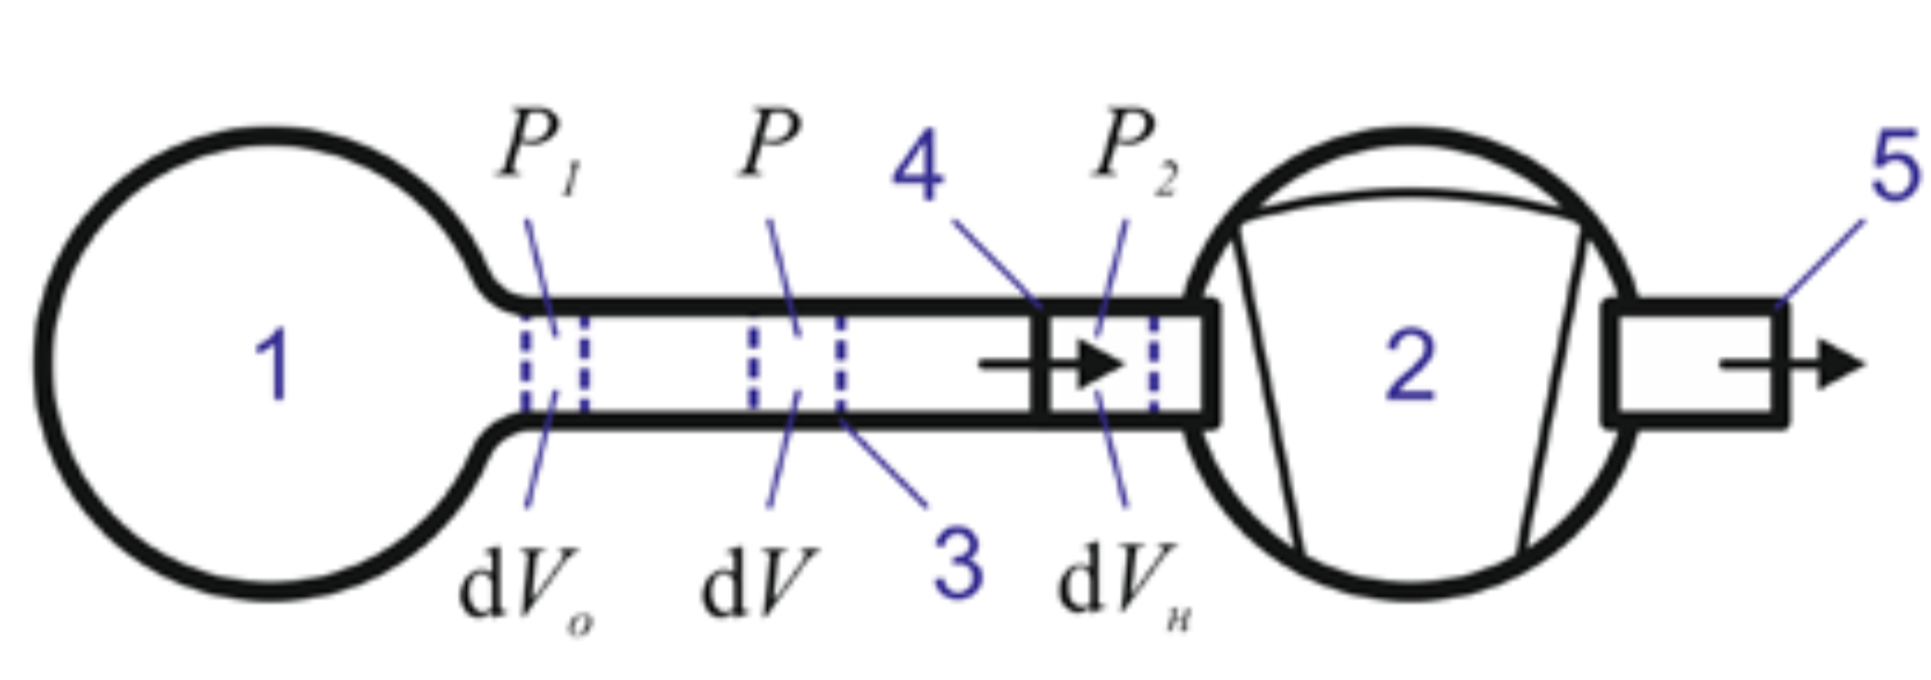
\includegraphics[width=\linewidth]{1}
    \caption{Зависимость числа $\alpha$-час\-тиц от глубины их
    проникновения в вещество}
    \label{fig:1}
\end{wrapfigure}

В формуле \eqref{eq:1} $R$ --- пробег $\alpha$-частица в воздухе (при
$15^\circ C$ и нормальном атмосферном давлении), выраженный в
сантиметрах, а энергия $E$ --- в мегаэлектрон-вольтах. Кроме величины
$R$, можно ввести величину $R' = \rho R$, где $\rho$ --- плотность
среды. $R'$ будем также называть пробегом.

Рассеяние $\alpha$-частиц в веществе и статистический характер потерь
энергии приводят к тому, что даже при одинаковой начальной энергии
пробеги разных $\alpha$-частиц несколько отличаются друг от друга. Это
различия проявляются в форме кривой, выражающей зависимость числа
частиц от расстояния, пройденного ими в поглотителе \ffig{fig:1}.

Как видно из кривой $d N/dx$, большая часть $\alpha$-частиц
останавливается в узкой области, расположенной около некоторого
значения $x$, которое называется средним пробегом $R_\text{ср}$. В
формулу \eqref{eq:1} входит $R_\text{ср}$. Также используют
экстраполированный пробег $R_\text{э}$. Из-за того, что мы имеем дело
не с узкими параллельными пучками частиц, а с пучками конечных
размеров, обладающими заметной угловой расходимостью более точное
значение будет давать не $R_\text{ср}$, а $R_\text{э}$.



\section{Эксперимент}

\begin{wrapfigure}[16]{l}{0.25\linewidth}
    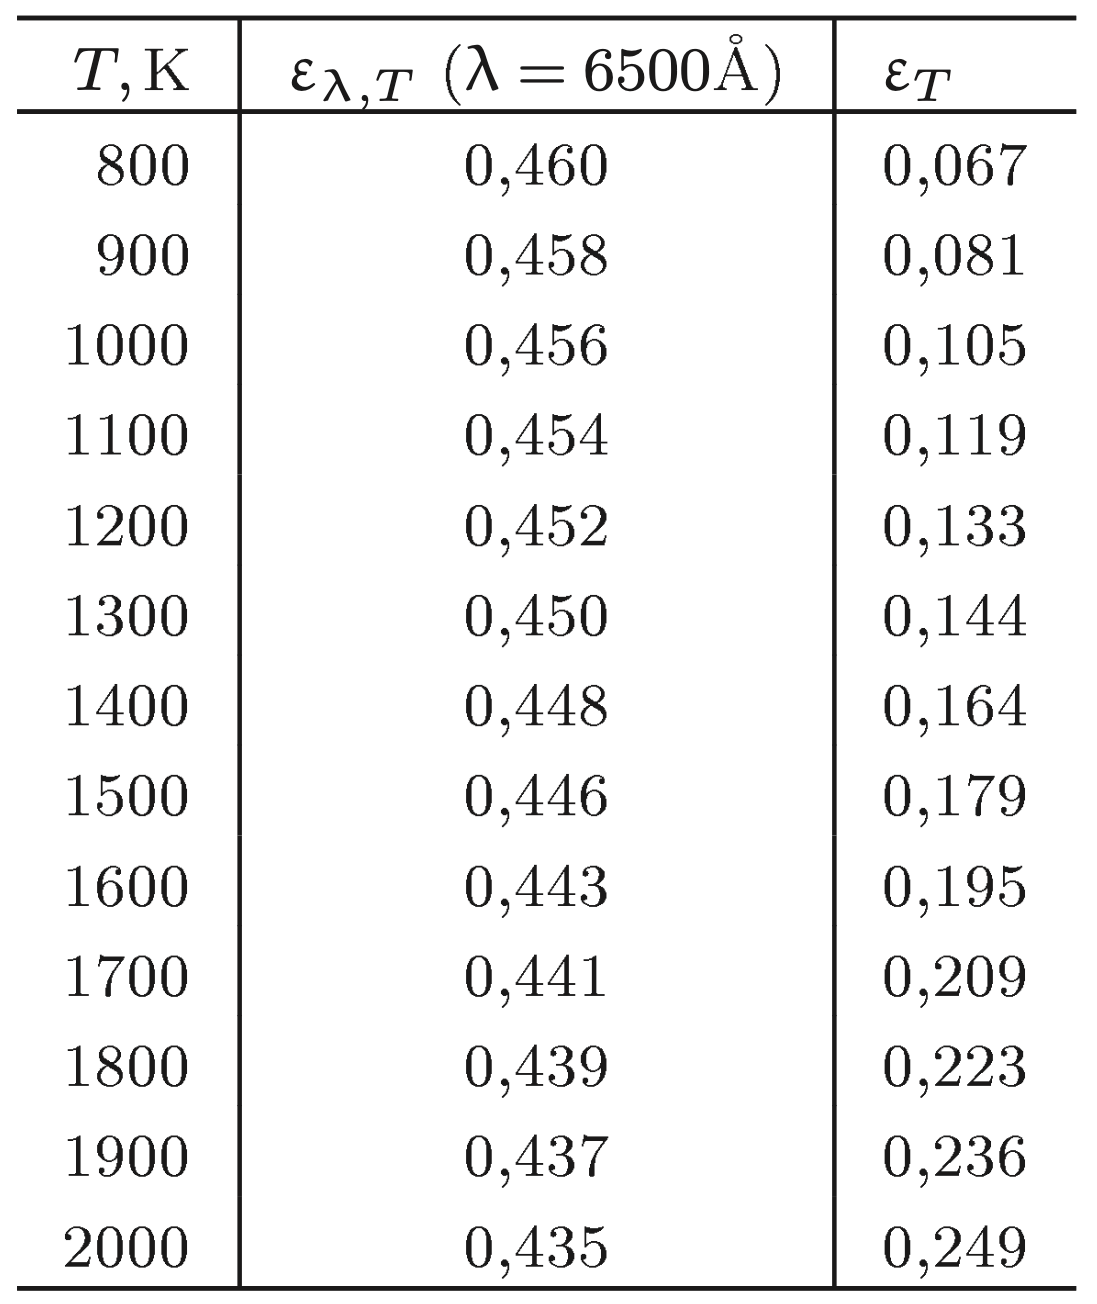
\includegraphics[width=\linewidth]{2}
    \caption{Установка для измерения пробега $\alpha$-частиц с помощью
    сцинтилляционного счетчика}
    \label{fig:2}
\end{wrapfigure}

В качестве источника $\alpha$-чатиц в работе используется
$^{239}\text{Pu}$. Альфа-частица, испускаемые $ ^{239}\text{Pu}$,
состоят из трех моноэнергетических групп, различие между которыми
лежит в пределах $50\: \text{кэВ}$. При той точности, которая
достигается в опыте, можно считать эти энергии совпадающими и равными
$5,15\:\text{МэВ}$.



\subsection{Экспериментальная установка}



\subsection*{Определение пробега $\symbf{\alpha}$-частиц с помощью
сцинтилляционного счетчика}

Установка состоит из цилиндрической камеры, на дне которой находится
исследуемый препарат. Камера герметично закрыта стеклянной пластинкой,
на которую с внутренней стороны нанесен слой люминофора. С наружной
стороны к стеклу прижат фотокатод фотоумножителя \ffig{fig:1}. Оптический контакт
ФЭУ-стекло обеспечивается тонким слоем вазелинового масла.

\begin{wrapfigure}[12]{r}{0.35\linewidth}
    \vspace{-10pt}
    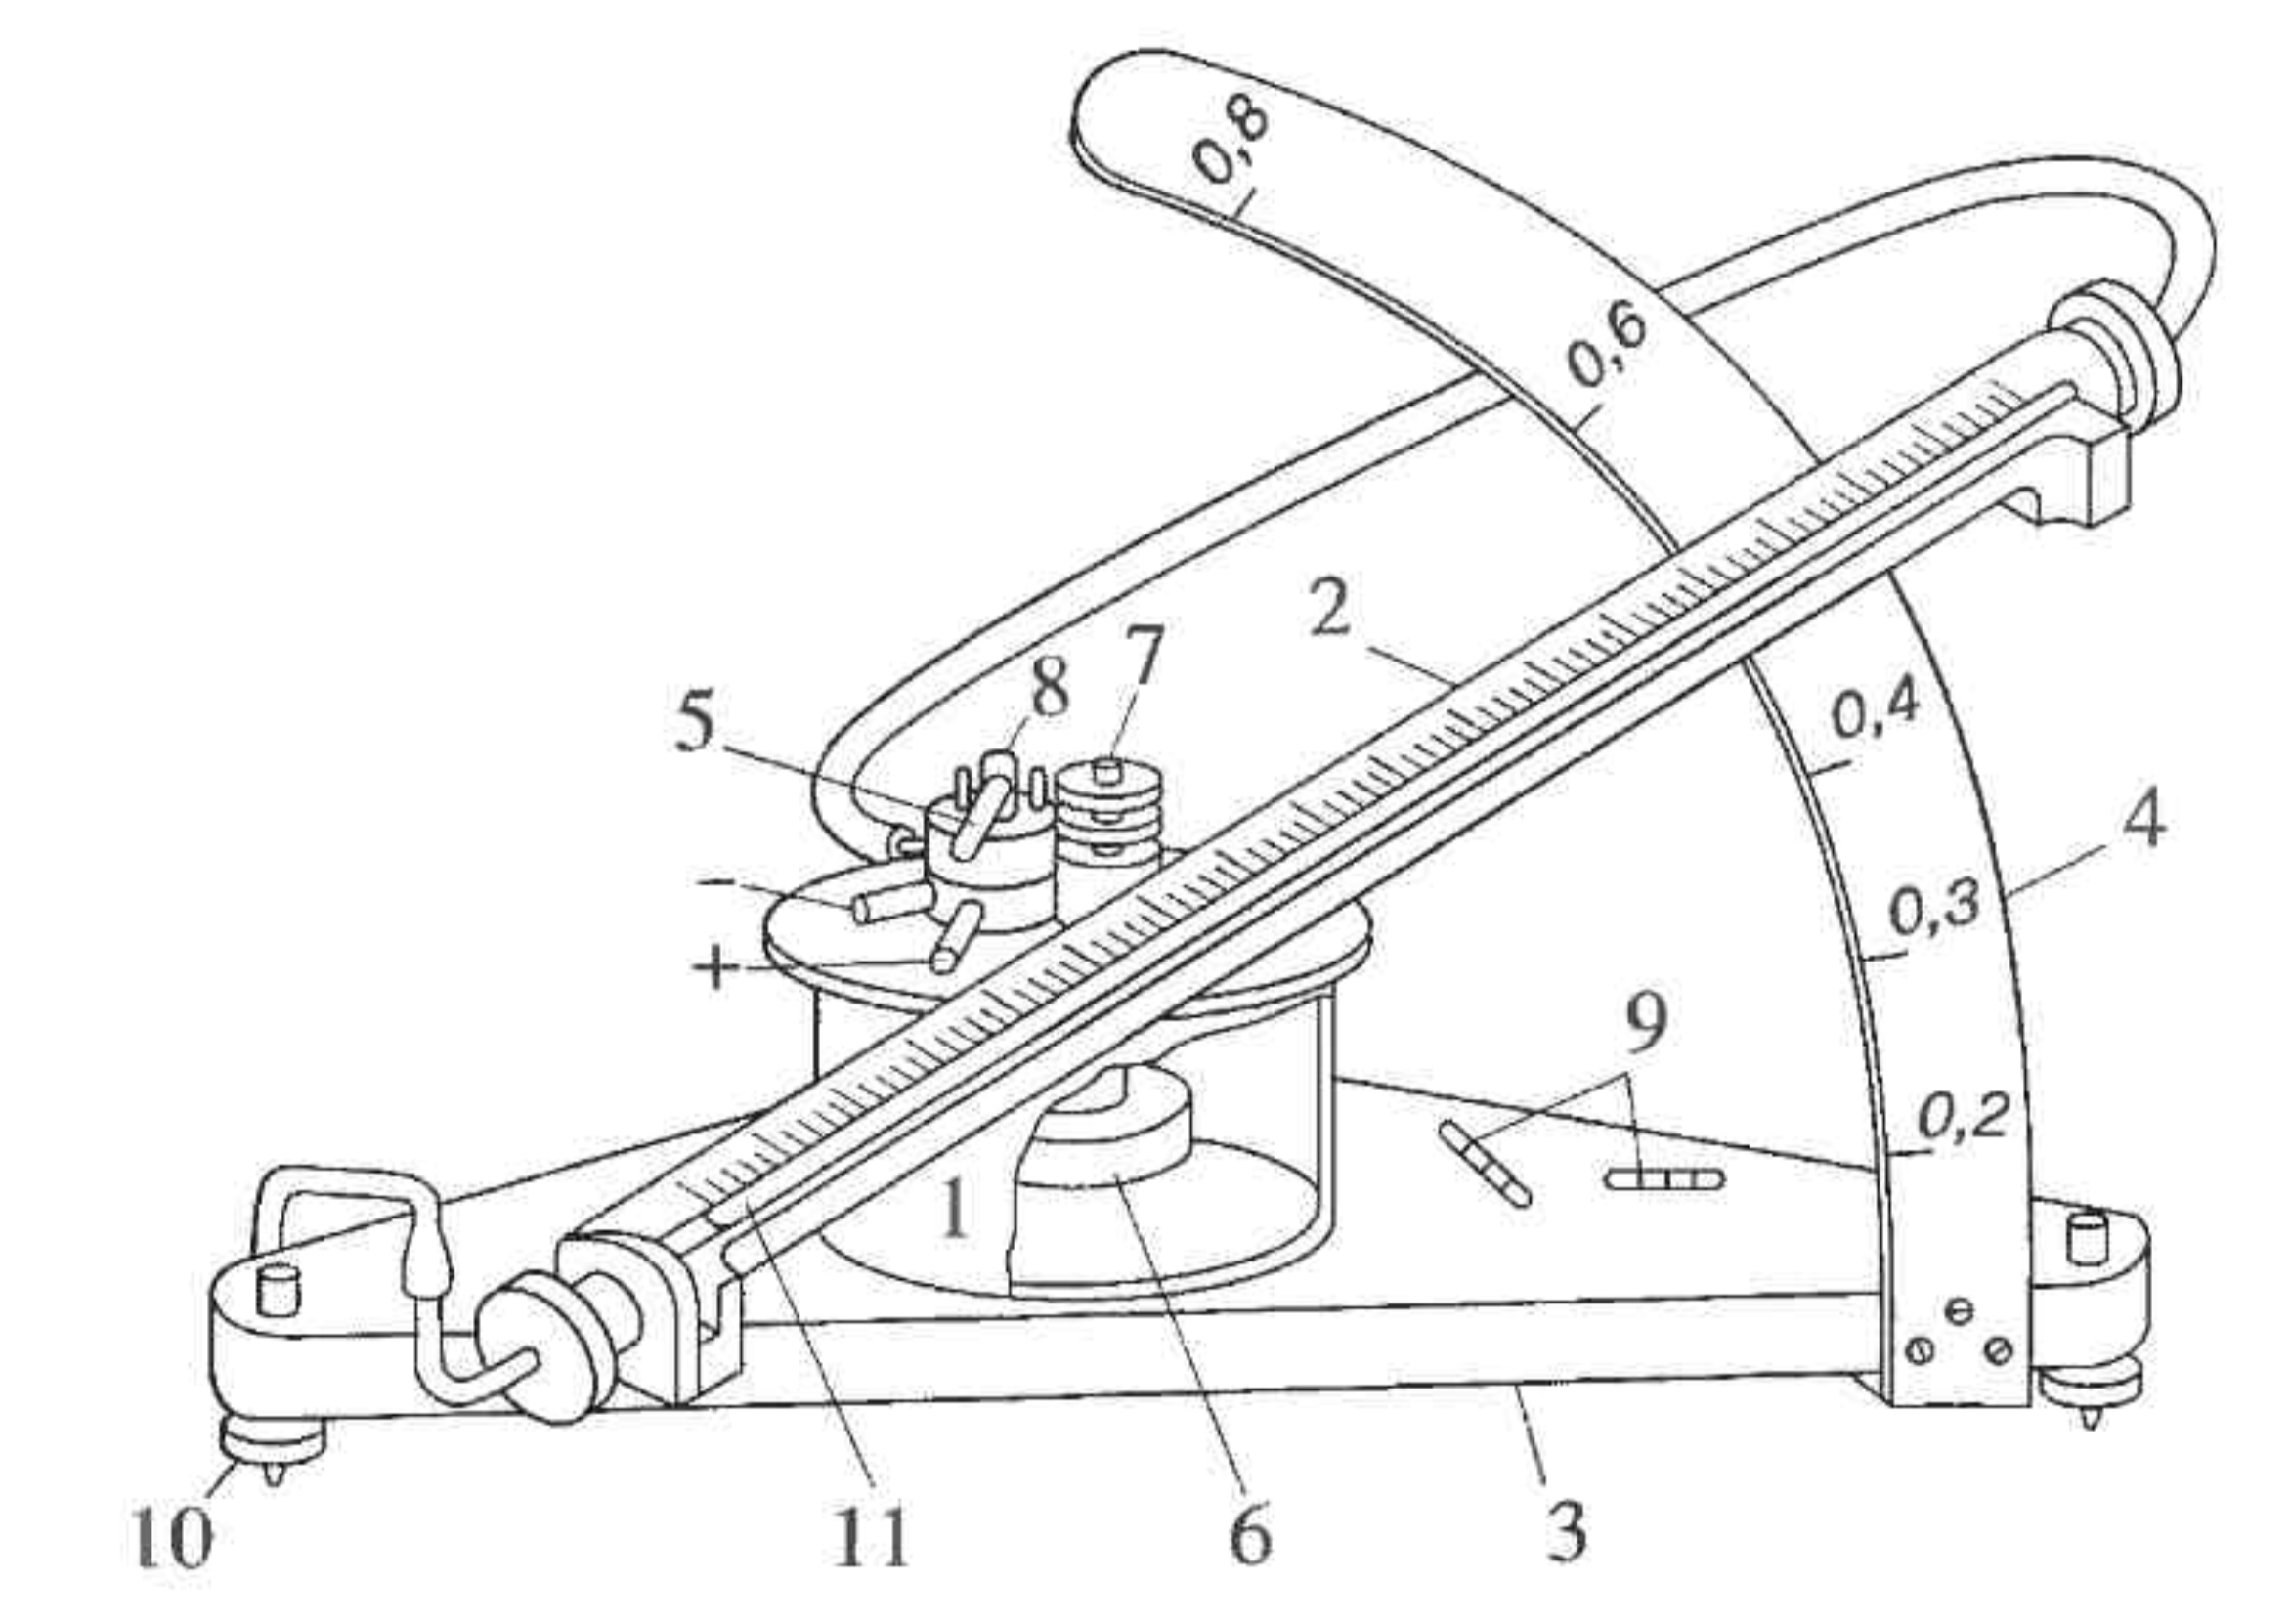
\includegraphics[width=\linewidth]{3}
    \caption{Схема устройства ионизационной камеры}
    \label{fig:3}
\end{wrapfigure}


Сигналы с фотоумножителя через усилитель поступают на переучетную
установку. Расстояние между препаратом и люминофором составляет $9\:
\text{см}$, так что $\alpha$-частицы не могут достигнуть люминофора
при обычном давлении. Определение пробега сводится к измерению
зависимости интенсивности счета от давления в камере.

\subsection*{Определение пробега $\symbf{\alpha}$-частиц с помощью
ионизационной камеры}
Ионизационная камера --- прибор для количественного измерения
ионизации, произведенной заряженными частицами при прохождении через
газ. Камера представляет собой наполненный газом сосуд  двумя
электродами (схема камеры приведена на \fig{fig:3}). Сферическая
стенка прибора служит одним из электродов, второй электрод вводится в
газ через изолирующую пробку. К электродам подводится постоянное
напряжение от источника ЭДС.

Ток возникает только при прохождении быстрой заряженной частицы,
которая рождает в газе на своем пути ионы. Ток, протекающий через
камеру, вначале будет резко возрастать, а затем, начиная с некоторого
напряжения $V_0$ станет постоянным, как показано на \fig{fig:4}. 

При небольшом напряжении сила тока оказывается заметно меньше $I_0$.
Это происходит в основном потому, что часть ионов успевает
рекомбинировать и не доходит до электродов камеры. При достаточно
больших напряжениях (порядка сотен вольт) ионы движутся достаточно
быстро, и рекомбинация не играет существенной роли. При использовании
камеры для регистрации ионизирующего излучения будет стремиться
работать в области плато, так как при этом сила тока не зависит от
небольших изменений напряжения на электродах камеры. 


\begin{figure}[H]
    \floatsetup{heightadjust=object,valign=c}
    \begin{floatrow}

        \ffigbox{
        \caption{Вольт-амперная характеристика ионизационной камеры}
    }
        {
        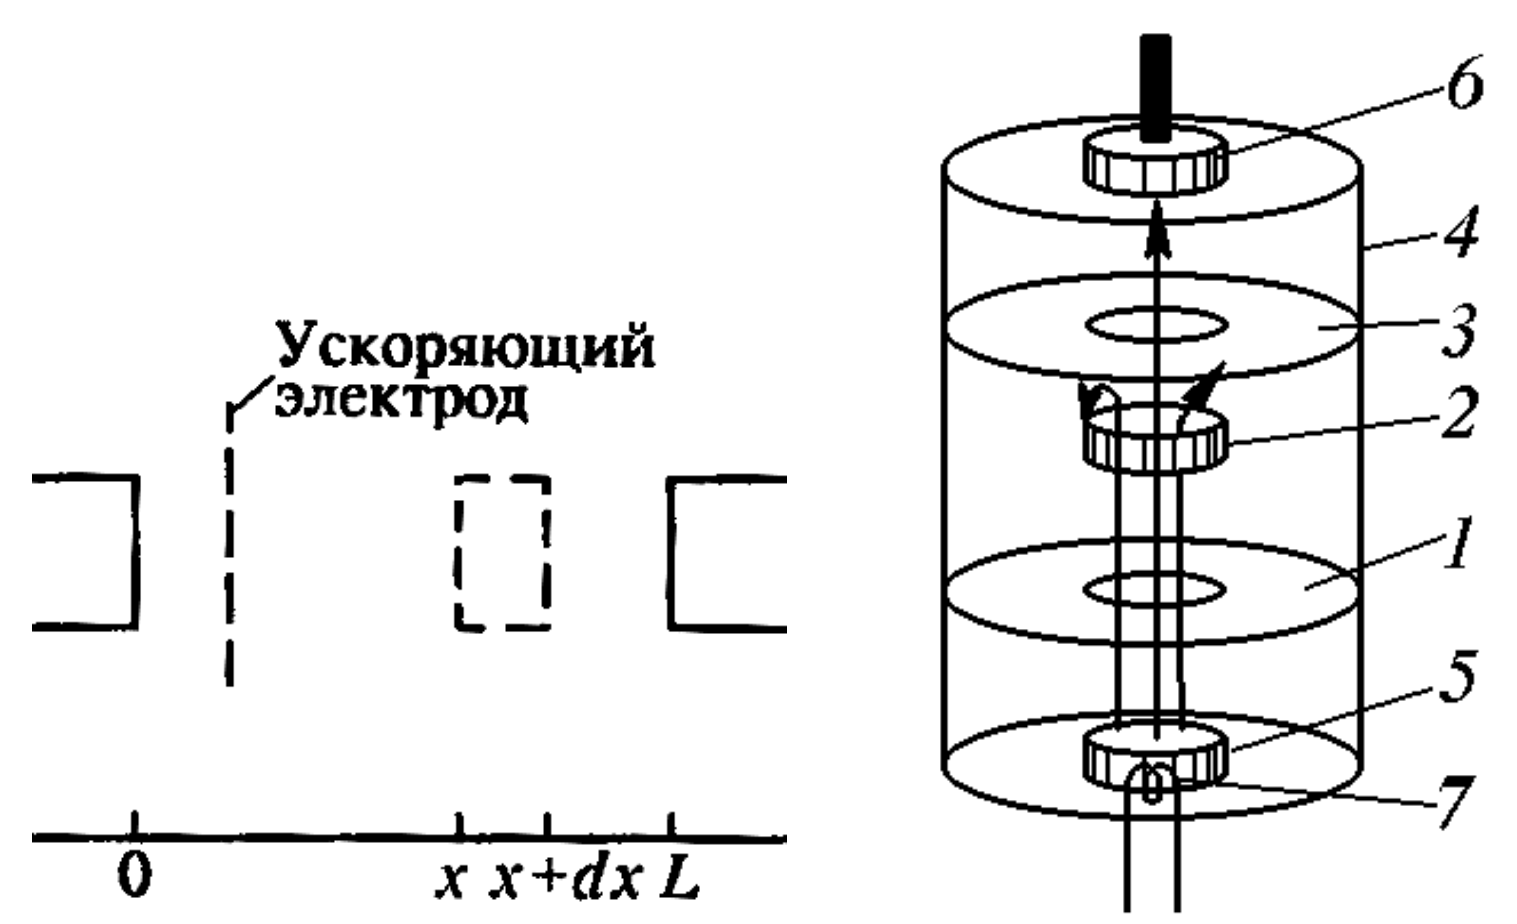
\includegraphics[width=0.5\linewidth]{4}
        \label{fig:4}
    }

        \ffigbox{
            \caption{Характерная кривая зависимости тока ионизационной
            камеры от давления. Ионизация создается $\alpha$-частицами}
    }
        {
        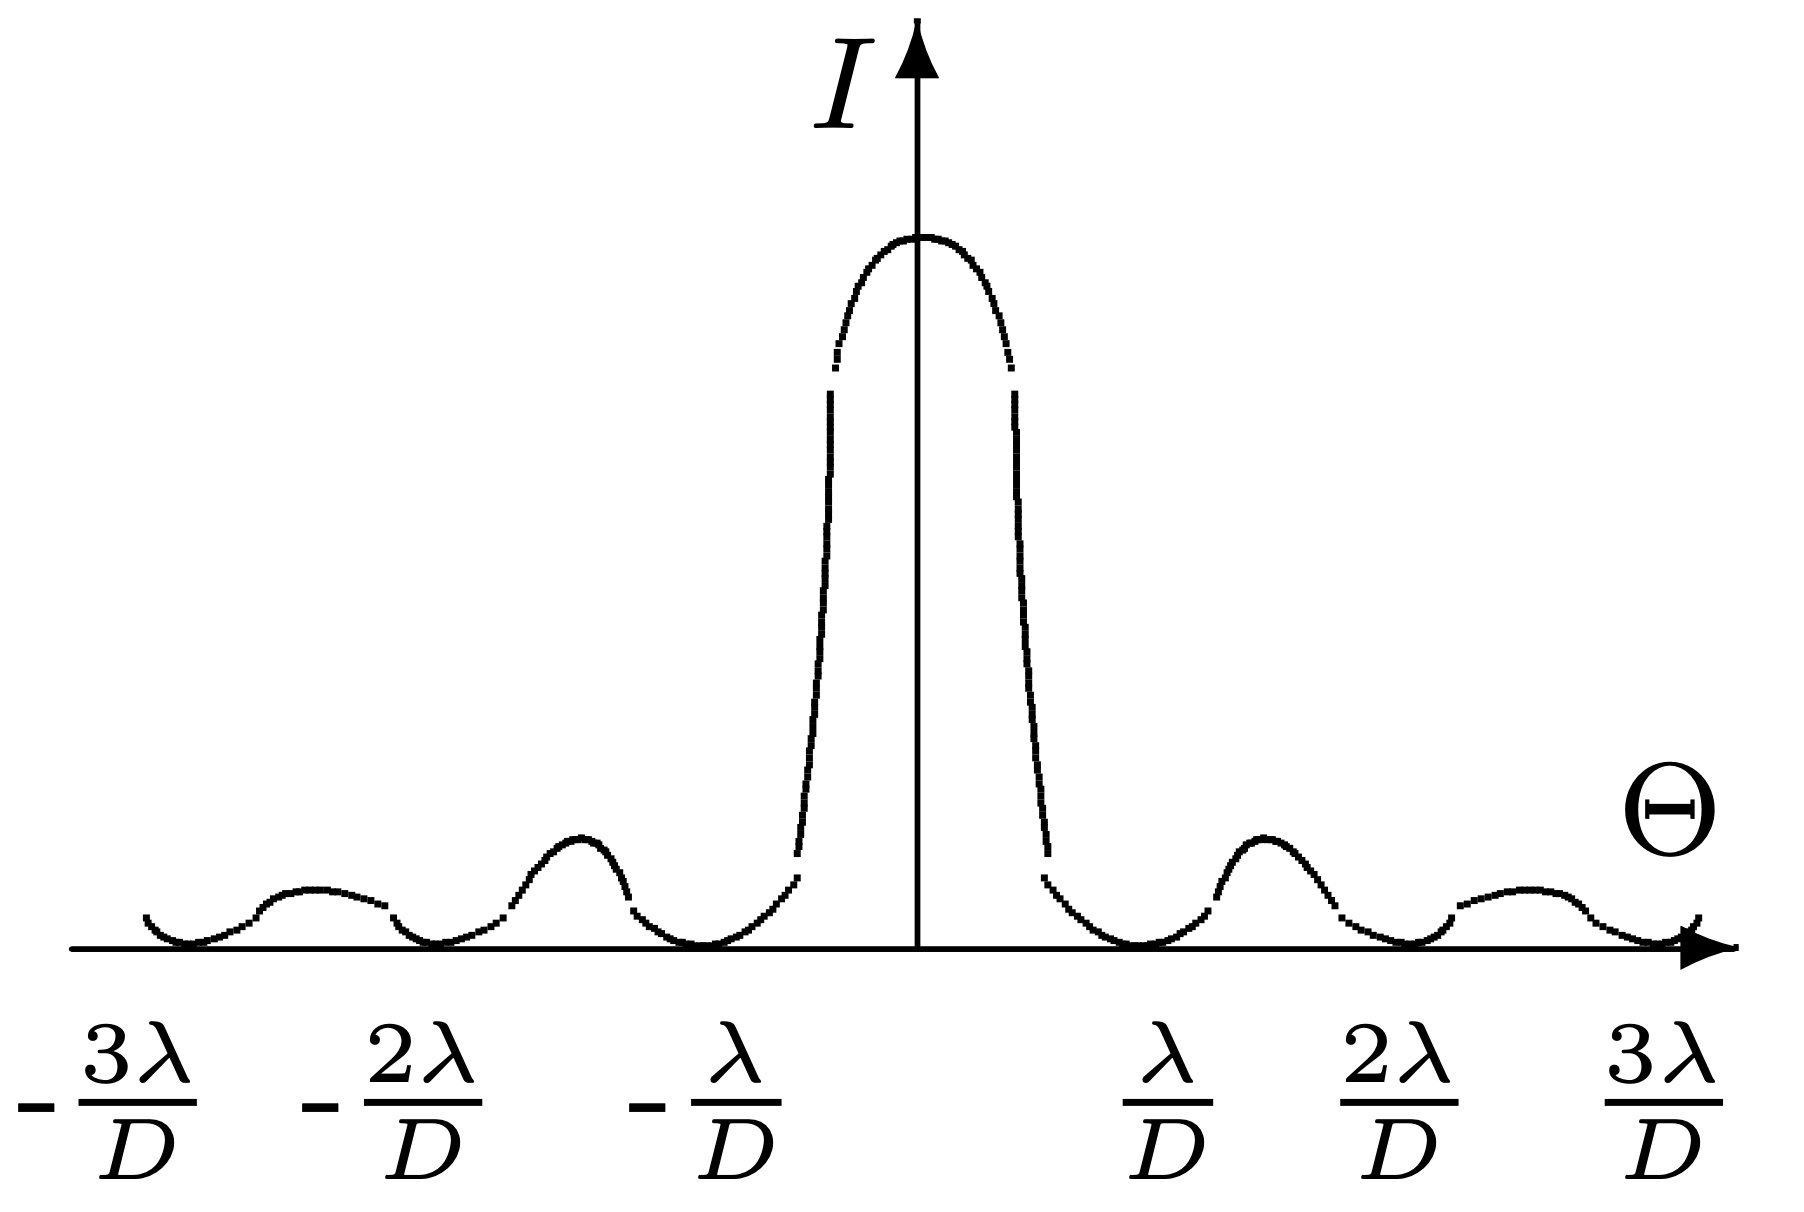
\includegraphics[width=0.5\linewidth]{5}
        \label{fig:5}
    }
    \end{floatrow}
\end{figure}

При изменении давления в камере ионизационный ток меняется так, как
это показано на \fig{fig:5}. При небольших давлений газа
$\alpha$-частицы передают часть энергии стенками камеры. По достижении
давления $P_0$ все они заканчивают свой пробег внутри газа, и
дальнейшее возрастание тока прекращается. 

В данной работе измерение пробега $\alpha$-частица проводится по
величине тока ионизации с сферической камере. Внутренним электродом
камеры служит диска диаметром $5\: \text{мм}$, на который нанесен
тонкий слой $ ^{239}_{94}\text{Pu}$, покрытый сверху тонкой защитной пленкой.
Вторым электродом служит внешняя оболочка камеры --- полый шар с
внутренним диаметром $100\: \text{мм}$. Оба электрода тщательно
изолированы друг от друга и от земли. 





\section{Результаты эксперимента}
\subsection*{Определение пробега $\symbf{\alpha}$-частиц с помощью
сцинтилляционного счетчика}
Проведем измерение зависимости счета частиц $N$ в секунду от давления $P$ в
камере. Построим график $N = N(P)$ \ffig{fig:6}, по которому
определяется средний и
экстраполированный пробег $\alpha$-частиц при условиях опыта --- $P_0
= 98,6\: \text{кПа}$, $t = 23^\circ C$.

\begin{figure}[H]
    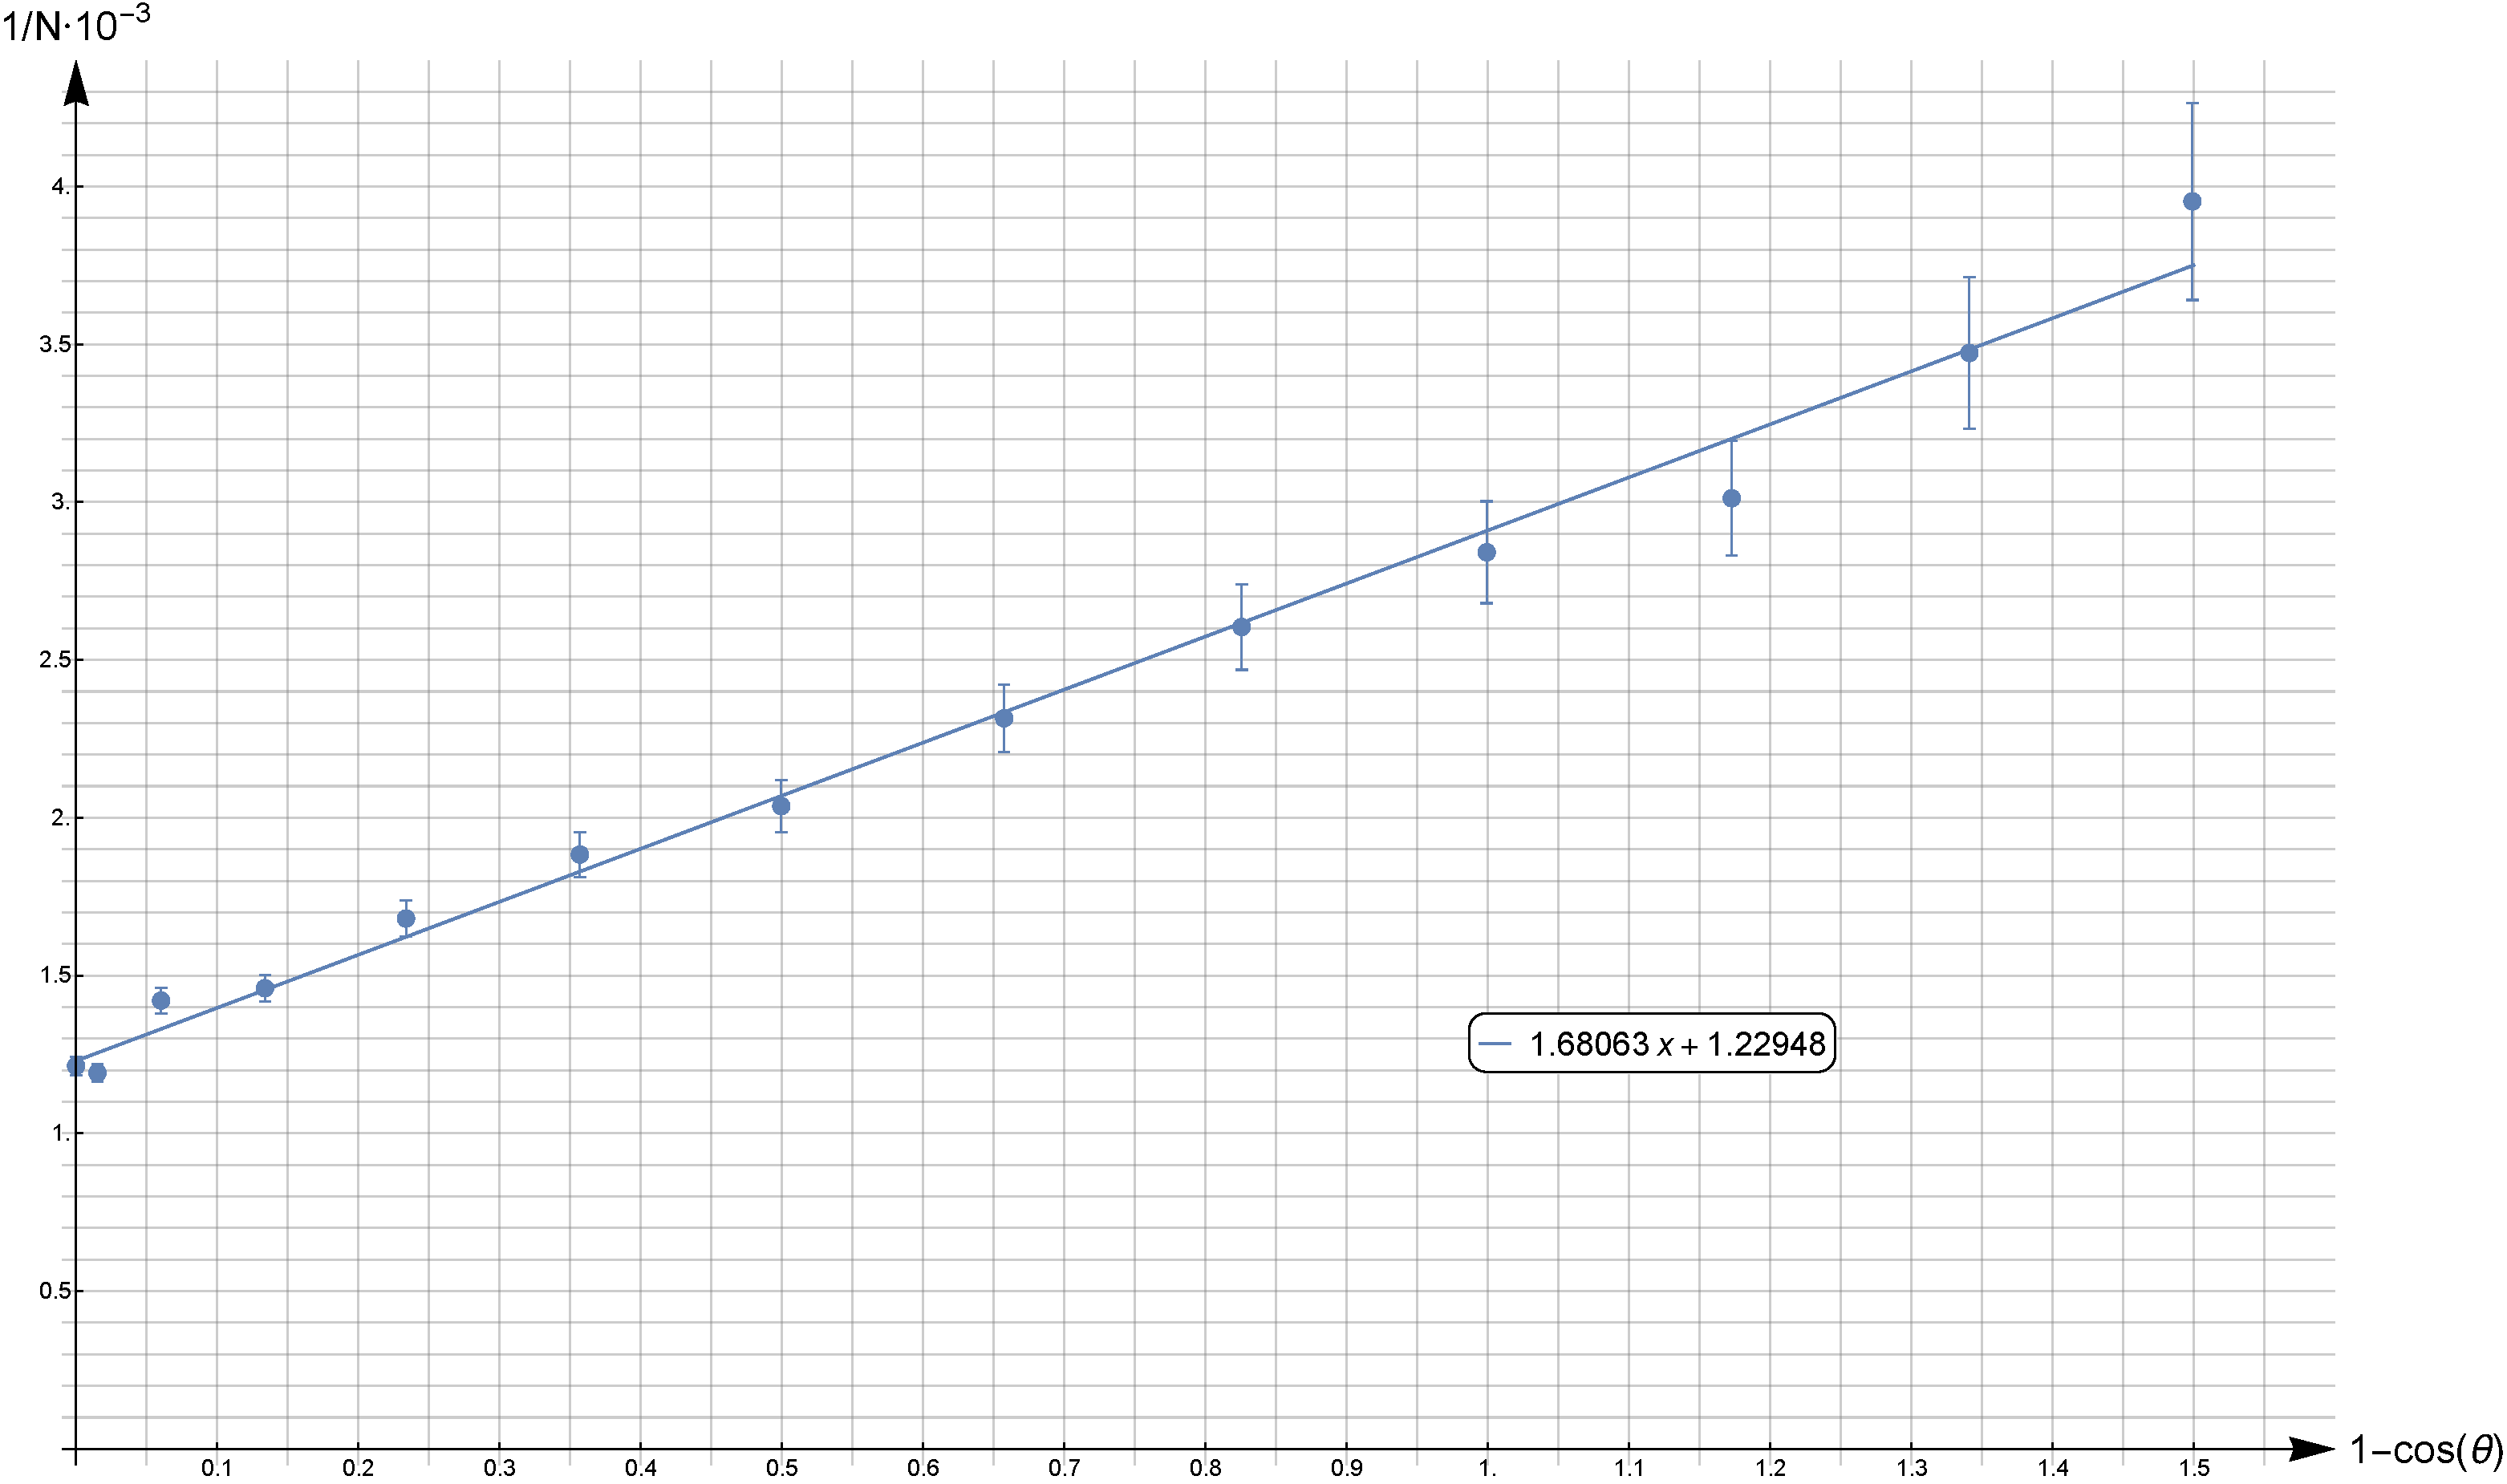
\includegraphics[width=0.9\linewidth]{6} 
    \caption{Зависимость количества сигналов с фотоумножителя в
    секунду $N$ от давления $P$}
    \label{fig:6}
\end{figure}

\subsection*{Определение пробега $\symbf{\alpha}$-частиц с помощью
ионизационной камеры}
Снимем зависимость тока через камеру $I$ от давления $P$:

\begin{figure}[H]
    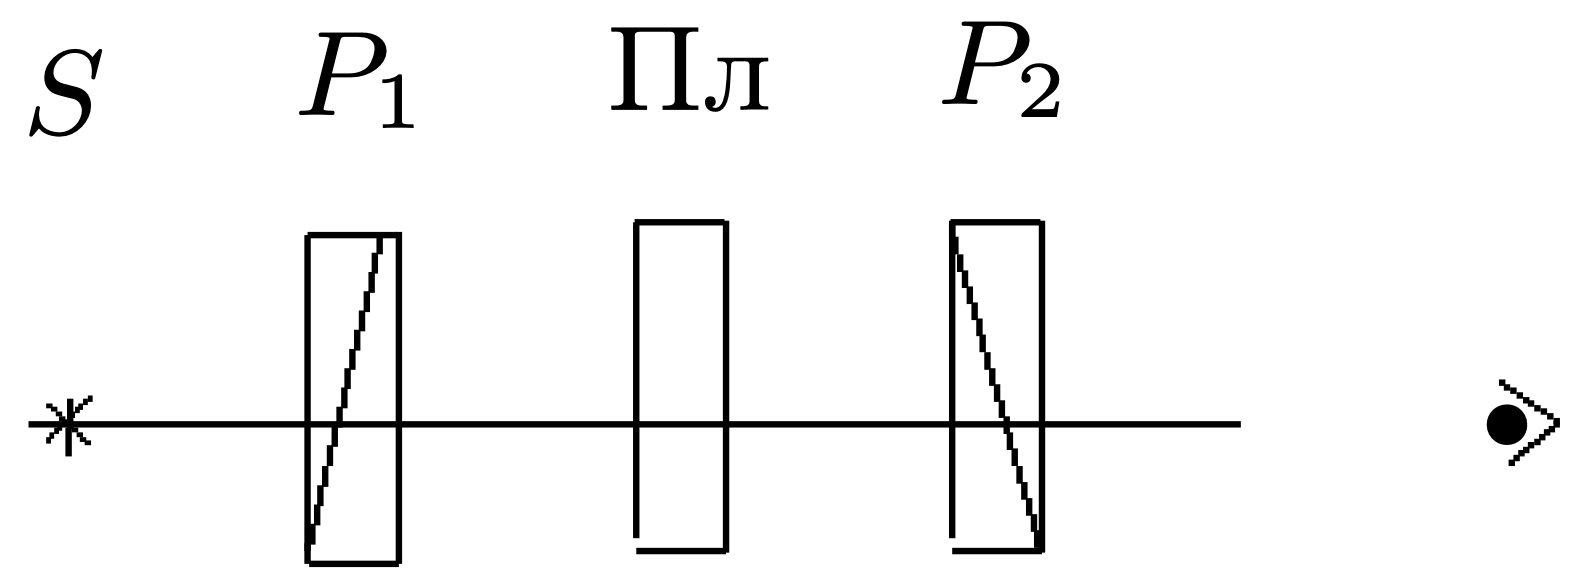
\includegraphics[width=0.9\linewidth]{7} 
    \caption{Зависимость тока через камеру $I$ от давления $P$}
    \label{fig:7}
\end{figure}




\section{Анализ результатов}
\subsection*{Определение пробега $\symbf{\alpha}$-частиц с помощью
сцинтилляционного счетчика}
Для вычисления длины свободного пробега будем использовать формулу
\begin{equation}
    R = \frac{k_B T}{\sqrt{2}\pi d^2 P}
    \label{eq:2}
\end{equation}
где $\pi d^2$ --- эффективная площадь поперечного сечения частиц.
Получим формулу для пересчета длины свободного пробега к другой
температуре и давлению:
\begin{equation}
    R_2 = \frac{T_1}{T_2} \frac{P_2}{P_1} R_1
    \label{eq:3}
\end{equation}

Выполним пересчет пробега к давлению $P = 760\: \text{Тор}$ и $T =
15^\circ C$, ответ выразим в см и в $\text{г}/\text{см}^2$. Плотность
воздуха при $T = 15^\circ C$ равна $1,2250\: \text{кг}/\text{м}^3$.
\begin{equation*}
    \begin{gathered}
        R_\text{э} =  (3,08 \pm 0,14)\: \text{см} = (3,8 \pm 0,2)\:
         \text{мг}/\text{см}^2\\
        R_\text{ср} =  (1,94 \pm 0,10)\: \text{см} = (2,38 \pm 0,12)\:
         \text{мг}/\text{см}^2
    \end{gathered}
\end{equation*}

По значениям $R_\text{э}$ и $R_\text{ср}$ определим толщину слюды
$\Delta h$,
закрывающей окно торцевого счетчика, при этом учтем, что пробег
$\alpha$-частицы в слюде, выраженный в $\text{г}/\text{см}^3$, в $1,2$
раза больше, чем пробег в воздухе, выраженный в тех же единицах.
\[
    \Delta h = (1,7 \pm 0,4)\: \text{г}/\text{см}^2
\]

Определим энергию $\alpha$-частиц по формуле \eqref{eq:1}, в формуле
будем использовать $R_\text{э}$.
\[
    E = (4,5 \pm 0,2)\: \text{МэВ}
\]

Зная период полураспада $^{239} \text{Pu}$ $T_{1/2} = 2,44 \cdot 10^4$ лет,
считая, что эффективность счета $\alpha$-частиц равна $100\%$ оценим
количество вещества в препарате. Телесный угол, под которым виден
источник, равен $0,04\: \text{ср}$.


Посчитаем начальное число атомов плутония $N_0$. Для вычисления числа
радиоактивных атомов в момент времени $T _{1/2}$ воспользуемся числом
$N$ при $P = 0$ на \fig{fig:6}. Это число возьмем приближенно равным
$350\: \text{c} ^{-1}$.
\begin{equation*}
    \begin{gathered}
        N_0 = 2 N(T _{1/2})\\
        N(T _{1/2}) = 350 \cdot \frac{2\pi}{0,04} \cdot T _{1/2}.
    \end{gathered}
\end{equation*}

Итого получим формулу для количества вещества в препарате $\nu$ и
вычислим значение:
\begin{equation*}
    \begin{gathered}
        \nu = \frac{N_0}{N_A} = \frac{2 \cdot 350 \cdot 2\pi \cdot T
        _{1/2}}{0,04 N_A}\\ 
        \nu \approx 1,4 \cdot 10 ^{-7}\: \text{моль}
    \end{gathered}
\end{equation*}


\subsection*{Определение пробега $\symbf{\alpha}$-частиц с помощью
ионизационной камеры}
Определим экстраполированный пробег $\alpha$-частиц в воздухе при
условиях опыта и выполним перерасчет к $P = 760\: \text{Тор}$, $T = 15
^{\circ} C$ по формуле \eqref{eq:3}. 
\[
    R^*_\text{э} = (3,17 \pm 0,09)\: \text{см} = (3,88 \pm 0,11)\:
    \text{мг}/\text{см}^2
\]

Определим энергию $\alpha$-частиц по формуле \eqref{eq:1}:
\[
    E^* = (4,61 \pm 0,09)\: \text{МэВ}
\]












\section{Выводы}
С помощью сцинтилляционного счетчика и ионизационной камеры в работе
был измерен пробег $\alpha$-частиц в воздухе:
\begin{equation*}
    \begin{gathered}
        R_\text{э} =  (3,08 \pm 0,14)\: \text{см} = (3,8 \pm 0,2)\:
         \text{мг}/\text{см}^2\\
    R^*_\text{э} = (3,17 \pm 0,09)\: \text{см} = (3,88 \pm 0,11)\:
    \text{мг}/\text{см}^2
    \end{gathered}
\end{equation*}

Значения в пределах погрешностей совпадают друг с другом. По длинам
свободного пробега была определена энергия $\alpha$-частиц:
\begin{equation*}
    \begin{gathered}
    E = (4,5 \pm 0,2)\: \text{МэВ}\\
    E^* = (4,61 \pm 0,09)\: \text{МэВ}
    \end{gathered}
\end{equation*}

Результат, полученный с помощью ионизационной камеры получился
точнее, однако он также отличаются от табличного значения:
\[
    E^\text{т} = 5,15\: \text{МэВ}
\]

Расхождения могут быть связаны с использованием эмпирической формулы
для подсчета энергии \eqref{eq:1}, а также с неточностью измерений.
При измерении с помощью сцинтилляционного счетчика неточность связана
с угловой расходимостью пучка $\alpha$-частиц, при измерении с помощью
ионизационной камеры неточность возникает в измерении малых токов.

По измеренным значениям среднего пробега и экстраполированного пробега
(с помощью сцинтилляционного счетчика)
была вычислена толщина слюды, закрывающей окно торцевого счетчика.
\[
    \Delta h = (1,7 \pm 0,4)\: \text{г}/\text{см}^2
\]

По периоду полураспада плутония $ ^{239} \text{Pu}$ была проведена
оценка количества вещества в препарате:
\[
        \nu \approx 1,4 \cdot 10 ^{-7}\: \text{моль}
\]


\section*{А. Приложение}
Данные для построения графика на \fig{fig:6}:

\renewcommand{\arraystretch}{1.4}
\begin{table}[H]
\centering
\begin{tabular}{|c|c|c|c|cc}
\hline
$P,\: \text{кПа}$    & $N,\: \text{с}^{-1}$     & $P,\: \text{кПа}$     & $N,\: \text{с}^{-1}$     & \multicolumn{1}{c|}{$P,\: \text{кПа}$}     & \multicolumn{1}{c|}{$N,\: \text{с}^{-1}$}    \\ \hline
0,00  & 364,5 & 19,72 & 215,4 & \multicolumn{1}{c|}{34,68} & \multicolumn{1}{c|}{22,2} \\ \hline
3,40  & 345,1 & 22,44 & 181,2 & \multicolumn{1}{c|}{36,04} & \multicolumn{1}{c|}{8,0}  \\ \hline
6,12  & 336,8 & 25,16 & 138,4 & \multicolumn{1}{c|}{37,40} & \multicolumn{1}{c|}{3,6}  \\ \hline
8,84  & 325,2 & 27,88 & 99,7  & \multicolumn{1}{c|}{38,76} & \multicolumn{1}{c|}{1,1}  \\ \hline
11,56 & 295,6 & 30,60 & 63,0  & \multicolumn{1}{c|}{44,20} & \multicolumn{1}{c|}{0,1}  \\ \hline
14,28 & 284,8 & 31,96 & 49,2  & \multicolumn{1}{c|}{57,80} & \multicolumn{1}{c|}{0,2}  \\ \hline
17,00 & 238,1 & 33,32 & 35,2  &                            &                           \\ \cline{1-4}
\end{tabular}
\caption{Зависимость количества сигналов с фотоумножителя в секунду
$N$ от давления $P$}
\end{table}

Данные для построения графика на \fig{fig:7}:

\begin{table}[H]
\centering
\begin{tabular}{|c|c|c|c|c|c|}
\hline
$P,\: \text{кПа}$     &  $I,\: \text{пА}$  & $P,\: \text{кПа}$     &
$I,\: \text{пА}$   & $P,\: \text{кПа}$     & $I,\: \text{пА}$   \\ \hline
0,00  & 8   & 65,96 & 835 & 79,56 & 951 \\ \hline
3,40  & 42  & 67,32 & 851 & 80,92 & 947 \\ \hline
17,00 & 188 & 68,68 & 875 & 82,28 & 946 \\ \hline
30,60 & 348 & 70,04 & 895 & 83,64 & 947 \\ \hline
44,20 & 522 & 71,40 & 908 & 85,00 & 935 \\ \hline
57,80 & 711 & 71,40 & 911 & 87,72 & 935 \\ \hline
59,16 & 733 & 72,76 & 928 & 90,44 & 932 \\ \hline
60,52 & 754 & 74,12 & 931 & 93,16 & 929 \\ \hline
61,88 & 772 & 75,48 & 941 & 95,88 & 924 \\ \hline
63,24 & 793 & 76,84 & 943 & 98,60 & 918 \\ \hline
64,60 & 816 & 78,20 & 946 & 99,28 & 913 \\ \hline
\end{tabular}
\caption{Зависимость тока через камеру $I$ до давления $P$}
\end{table}








\end{document}
